\section{Week 4}
\begin{center}
    \textbf{\large \underline{$\bm{\mathcal{Z}}$-Transform}}
\end{center}

\textbf{\large \underline{$\mathcal{Z}$ - $\mathcal{S}$ Conversion}}
\begin{itemize}
    \item Matched Z-transform Method / Matched Dynamics Method / pole–zero mapping / Pole–Zero Matching Method: 
    \begin{equation*}
        z = e^{sT}
    \end{equation*}
    \item \textbf{\underline{Hidden Zero Method}} When you have to transfer a \textbf{TF} from s-domain to z-domain while excluding the \textbf{ZOH}, you can't use 'c2d()' or 'c2dm()' because these commands automatically include the \textbf{ZOH} to your \textbf{TF}. In that case, you have to do the conversion by hand. The following rules are observations grounded on Kahoot experiences and may be (or likely to be) wrong. 
    \begin{itemize}
        \item hidden zero $\eqdef \color{red} (s+\infty)$.
        \item $\color{red} e^{-\infty T} = -1$.
        \item \# of hidden zero = Order(den) - Order(num)
        \begin{itemize}
            \item Case 1: \# of hidden zero = 0 $\to$ use matched dynamics method;
            \item Case 2: \# of hidden zero $> 0$ $\to$ add these many hidden zeros;
            \item Case 3: \# of hidden zero $< 0$ $\to$ non-physical system.
        \end{itemize}
        \item Example: Find discrete equivalent of $G(s)=\frac{4}{s(s+4)}$ given that $T=0.02$.
        \begin{itemize}
            \item \# of hidden zero $= 2 - 0 =2$,
            \begin{align*}
                G(s) &= \frac{4\cdot \color{red}(s-(-\infty))\cdot \color{red}(s-(-\infty))}{(s-0)(s-(-4))} \\
                G(z) &= \frac{K_d \cdot  (z-\color{red} e^{-\infty T}\color{black})\cdot(z-\color{red} e^{-\infty T}\color{black}) }{(z-e^{(0+j0)T})(z-e^{(-4+j0)T})} \\
                &= \frac{K_d \cdot (z+\color{red}1 \color{black})^2 }{(z-1)(z-0.92312)} 
            \end{align*}
            \item Find $K_d$ by matching DC Gain.
\begin{lstlisting}
>> s=1e-12; % cause analytical DCG doesn't exist
>> Gs = 4/(s*(s+4));
>> T=0.02;
>> z=exp(s*T);
>> Gz=(z+1)^2/((z-1)*(z-0.92312));
>> K=Gs/Gz
>> K = 3.840927575993151e-04
\end{lstlisting}
        \end{itemize}
    \end{itemize}
    
    \item $\bm{\mathcal{Z}\Longleftrightarrow\;}$\textbf{discrete time} by hand (and tables)
    \begin{align*}
        y(k+2) + y(k+1) + y(k) - y(k-1) &= u(k) \\
        \xrightarrow{\mathcal{Z}} z^2 Y(z) + zY(z) + Y(z) - z^{-1} Y(z) &= U(z)
    \end{align*}
    \item $\bm{\mathcal{Z}\Longleftrightarrow\;}$\textbf{discrete time} by almighty \textbf{Wolfram Alpha}: 
    
    Type \textit{"inverse Z transform calculator"} 
    
    or \textit{"Z transform calculator"} in the search bar.
\end{itemize}






\textbf{\large Transfer function of ZOH}
\begin{equation*}
    G_{ZOH}(s) = \frac{1-e^{-sT}}{s} 
\end{equation*}

\textbf{\large TF of ZOH + Analogy System (ZAS)}
\begin{align*}
    G_{ZAS}(z) &= \mathcal{Z}\left\{\frac{1-e^{-sT}}{s}G_{p}(s)\right\} \\
    &=  (1-z^{-1})\mathcal{Z}\left\{\frac{G_p (s)}{s}\right\} \\
    &= \frac{z-1}{z} \mathcal{Z}\left\{\frac{G_p (s)}{s}\right\}
\end{align*}

\textbf{\large Trick for finding inverse $\mathcal{Z}$-transform}

Divide the expression by z first, then find inverse using tables.

Example:
\begin{align*}
    Y(z) &= \frac{z^2}{(z-1)(z-0.5) } \\
    \frac{Y(z)}{z} &= \frac{z}{(z-1)(z-0.5)} = \frac{2}{z-1} - \frac{1}{z-0.5} \\
    Y(z) &= \frac{2z}{z-1} - \frac{z}{z-0.5} \\
    y(k) &= \mathcal{Z}^{-1}\left\{\frac{2z}{z-1}\right\} - \mathcal{Z}^{-1}\left\{ \frac{z}{z-0.5}\right\} \\
    &= 2 - 0.5^{k}
\end{align*}

\textbf{\large Associativity of Continuous Transfer Functions}
\begin{figure}[H]
    \centering
    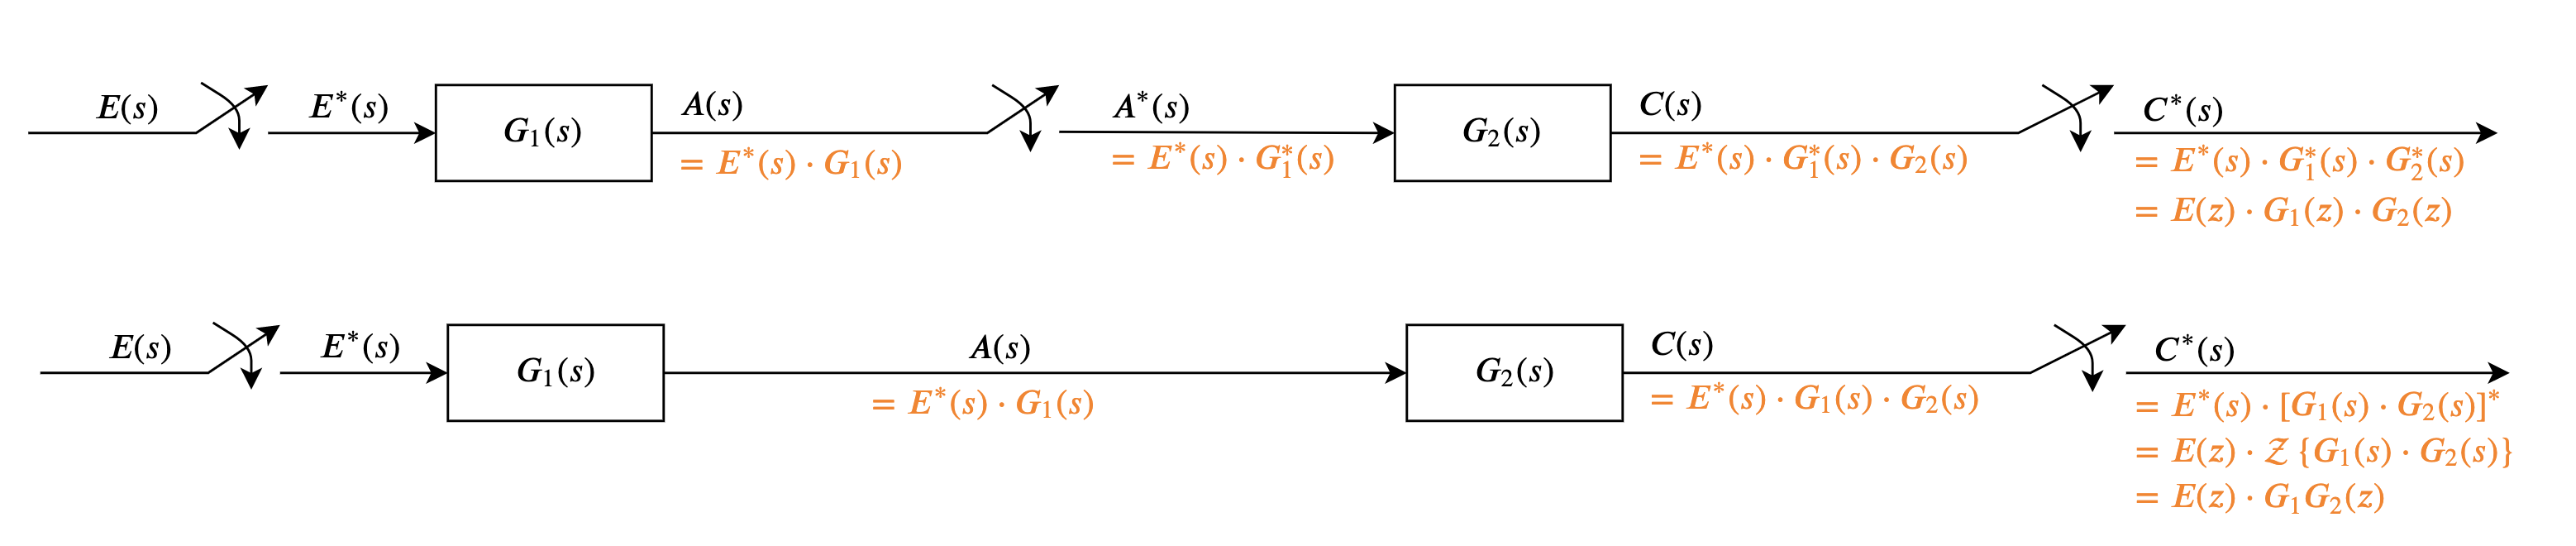
\includegraphics[width=0.5\textwidth]{images/associativity.png}
\end{figure}
Be careful: only distribute the * sign among addition/subtraction!

